\documentclass[11pt,a4paper]{article}
\usepackage[utf8]{inputenc}
\usepackage[T1]{fontenc}
\usepackage[french]{babel}
\usepackage{graphicx}
\usepackage{geometry}
\geometry{a4paper, margin=2cm}
\usepackage{hyperref}
\usepackage{float}

\begin{document}

\begin{titlepage}
    \centering
    \vspace*{2cm}
    
    {\scshape\LARGE Université de Montpellier \par}
    \vspace{1.5cm}
    {\scshape\Large Master 1 - Programmation Mobile\par}
    \vspace{2cm}
    
    \rule{\linewidth}{0.5mm} \\[0.6cm]
    {\Huge\bfseries Projet : Application Traveling\par}
    \vspace{0.5cm}
    {\Large\itshape Rendu Final : Analyse Fonctionnelle et Maquettes Complètes\par}
    \rule{\linewidth}{0.5mm} \\[2cm]
    
    \vspace{1.5cm}
    
    {\Large\bfseries Présenté par :}\\[0.8cm]
    {\LARGE AMMARI Reda \\ ALJIBBAOUI Tala \par}
    
    \vfill
    
    {\large \today\par}
\end{titlepage}

\newpage


\section{Analyse Fonctionnelle : Diagramme de Cas d'Utilisation}
Le diagramme de cas d'utilisation ci-dessous présente la structure globale de l'application "Traveling", divisée en deux modules interactifs : TravelShare (partage de contenu) et TravelPath (génération de parcours personnalisés). Les interactions avec les API externes (Météo, Réservation, IA) sont également modélisées.

\begin{figure}[H]
    \centering
    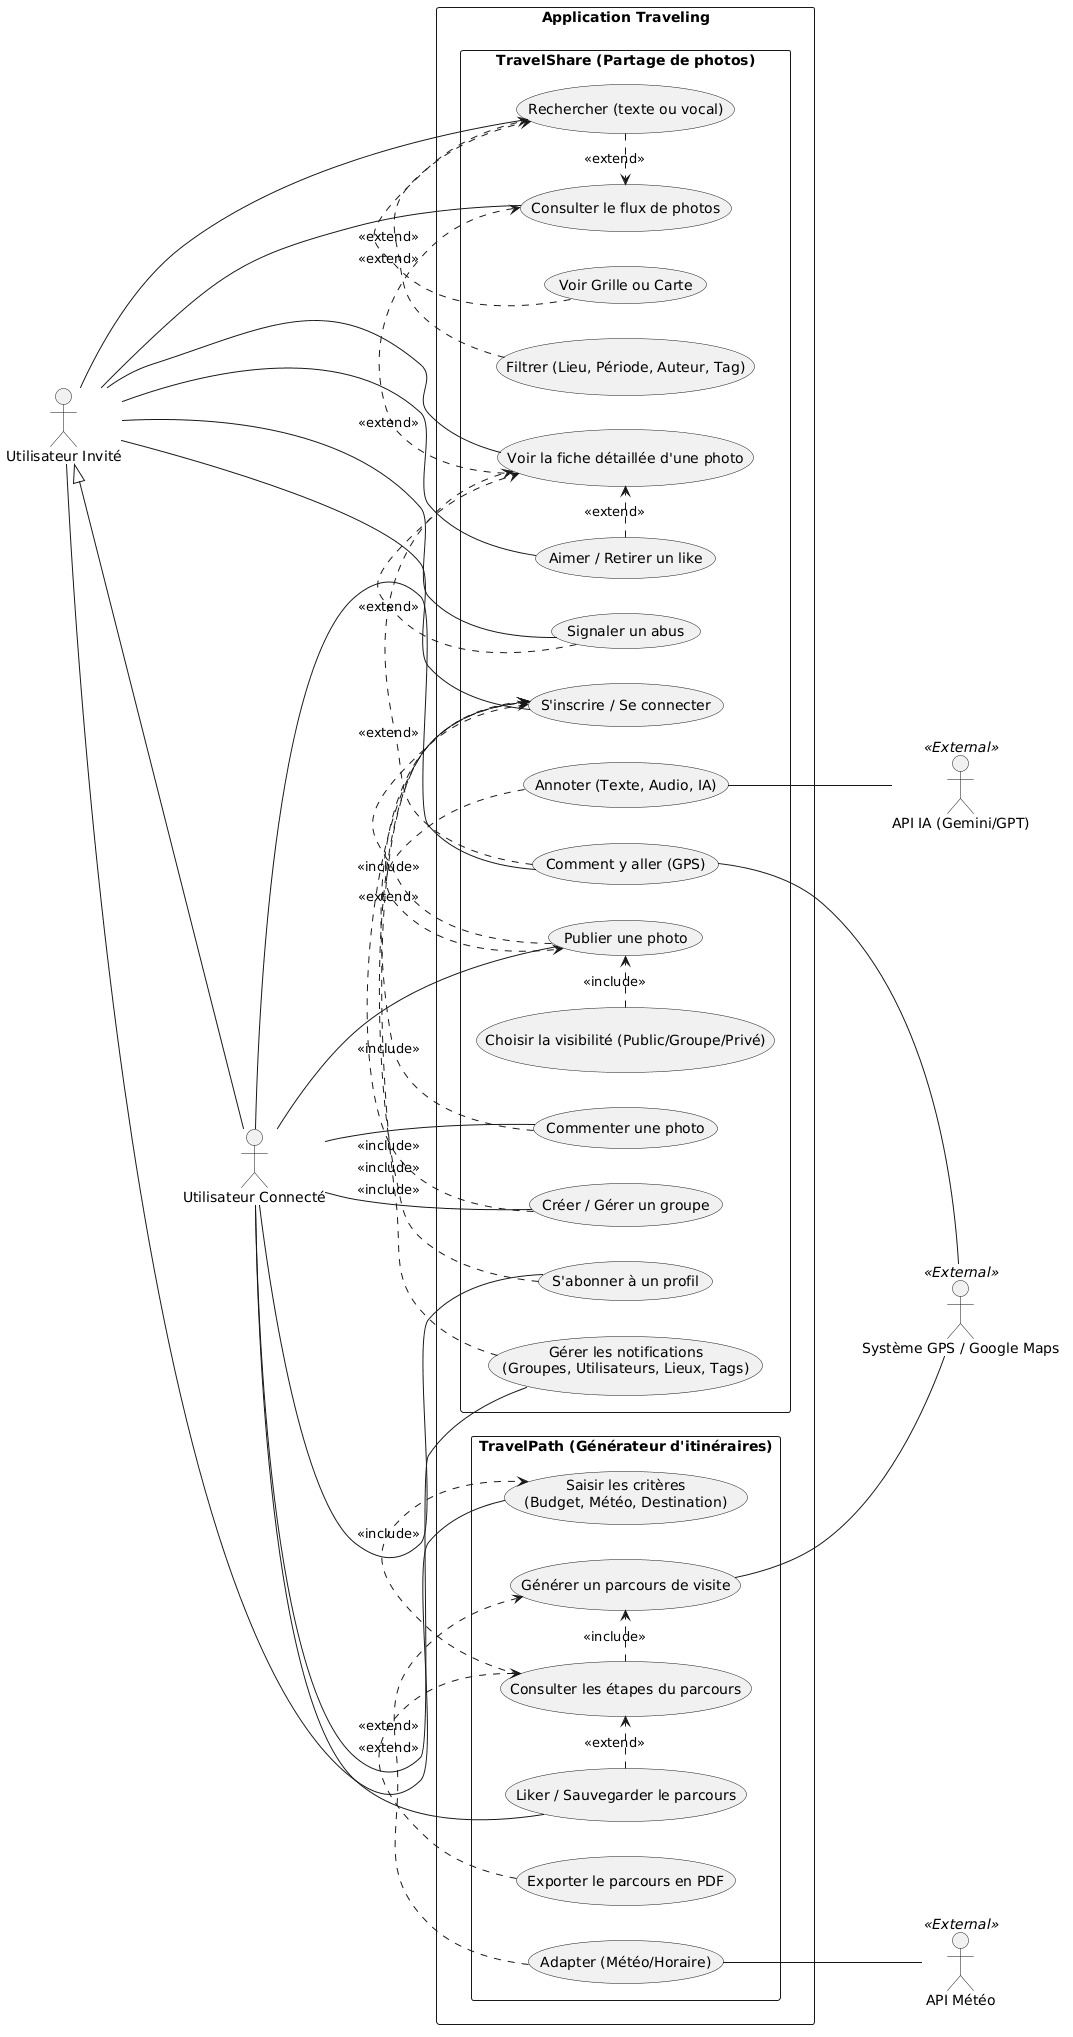
\includegraphics[width=\textwidth,height=0.8\textheight,keepaspectratio]{NewUML.png}
    \caption{Diagramme de cas d'utilisation global (TravelShare et TravelPath)}
\end{figure}

\newpage
\section{Maquettes de l'Application (React / Tailwind)}
Cette section présente les écrans finaux de l'application agencés pour une vue mobile optimale. Le design couvre l'intégralité des spécifications du sujet, incluant les fonctionnalités de mode connecté/non connecté, les groupes, et les trajets enregistrés.

\subsection{L'Authentification et L'Accueil (La Passerelle)}
L'écran principal de l'application sert de point d'entrée unique entre la partie réseau social et l'outil planificateur. Le système robuste d'authentification gère les droits et visibilités.

\begin{figure}[htbp]
    \centering
    \begin{minipage}{0.31\textwidth}
        \centering
        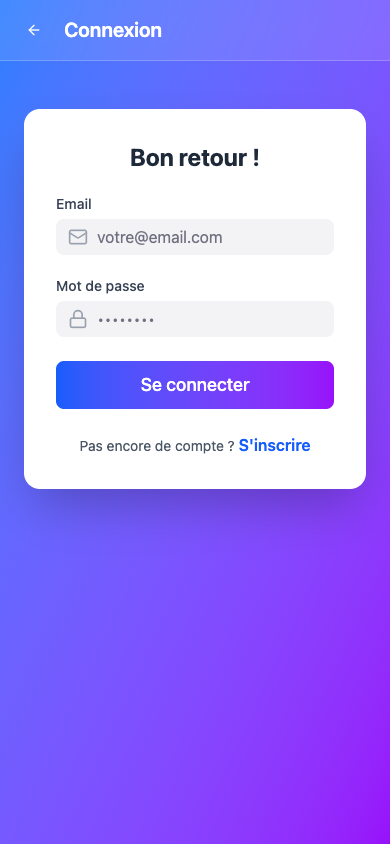
\includegraphics[width=0.95\textwidth]{sc_login.png}
        \caption{Connexion}
    \end{minipage}\hfill
    \begin{minipage}{0.31\textwidth}
        \centering
        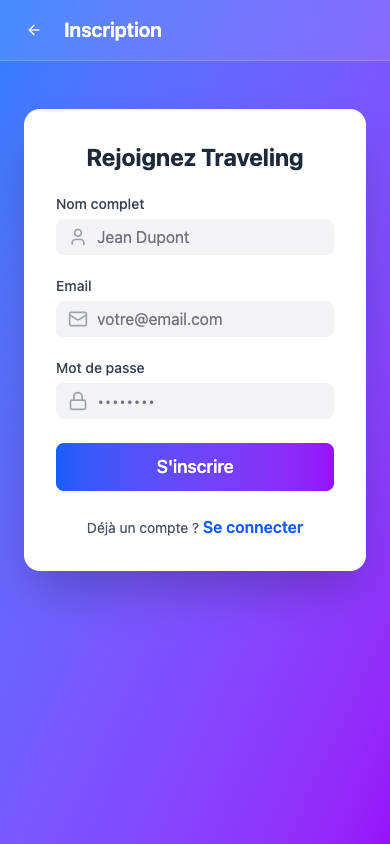
\includegraphics[width=0.95\textwidth]{sc_register.png}
        \caption{Inscription}
    \end{minipage}\hfill
    \begin{minipage}{0.31\textwidth}
        \centering
        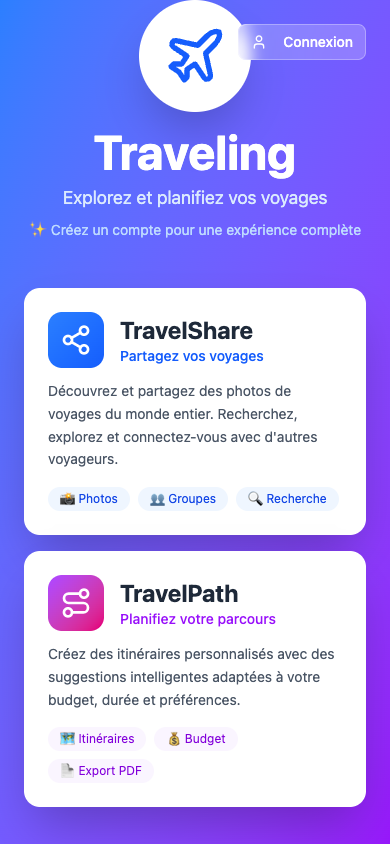
\includegraphics[width=0.95\textwidth]{sc_home.png}
        \caption{Accueil}
    \end{minipage}
\end{figure}

\subsection{TravelShare : Réseau Social et Groupes}
Le flux de photos interactif de la communauté avec les espaces dédiés aux groupes (TravelGroups) et le profil utilisateur regroupant les parcours enregistrés.

\begin{figure}[htbp]
    \centering
    \begin{minipage}{0.31\textwidth}
        \centering
        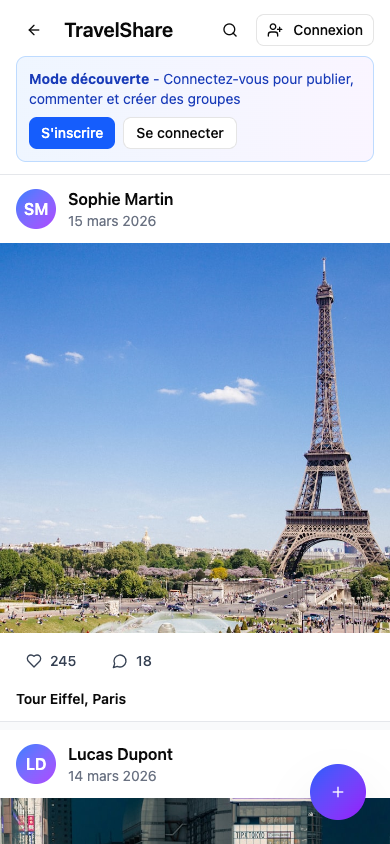
\includegraphics[width=0.95\textwidth]{sc_travelshare.png}
        \caption{Flux public}
    \end{minipage}\hfill
    \begin{minipage}{0.31\textwidth}
        \centering
        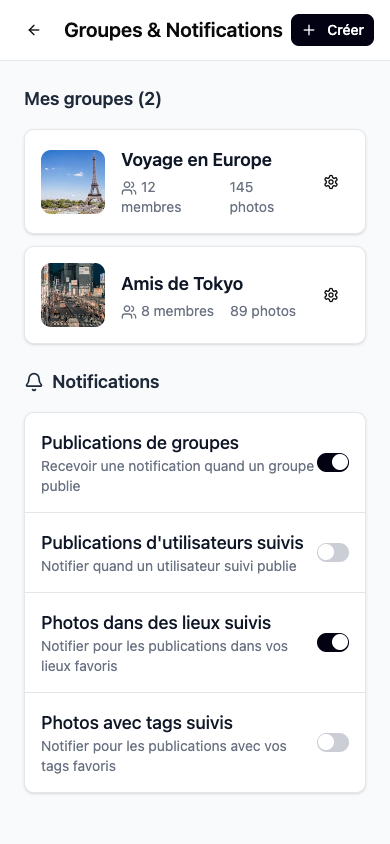
\includegraphics[width=0.95\textwidth]{sc_groups.png}
        \caption{Groupes}
    \end{minipage}\hfill
    \begin{minipage}{0.31\textwidth}
        \centering
        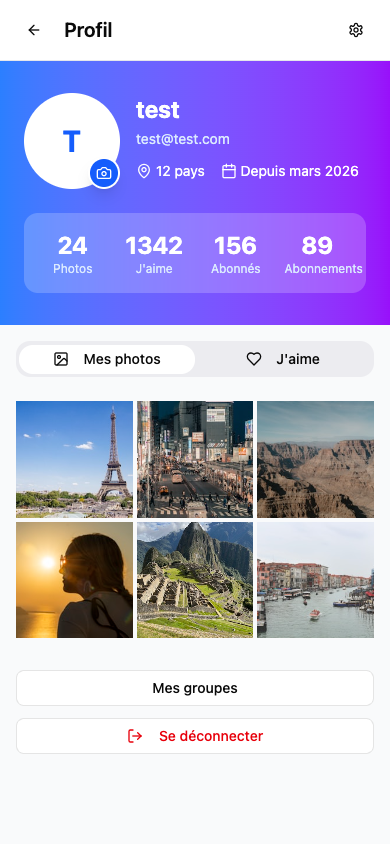
\includegraphics[width=0.95\textwidth]{sc_profile.png}
        \caption{Profil / Trajets}
    \end{minipage}
\end{figure}

\subsection{TravelPath : Planificateur d'Itinéraires}
Le formulaire intelligent permettant de paramétrer les attentes pour la génération automatique d'un itinéraire de voyage sur mesure, les options générées et le détail du trajet.

\begin{figure}[htbp]
    \centering
    \begin{minipage}{0.31\textwidth}
        \centering
        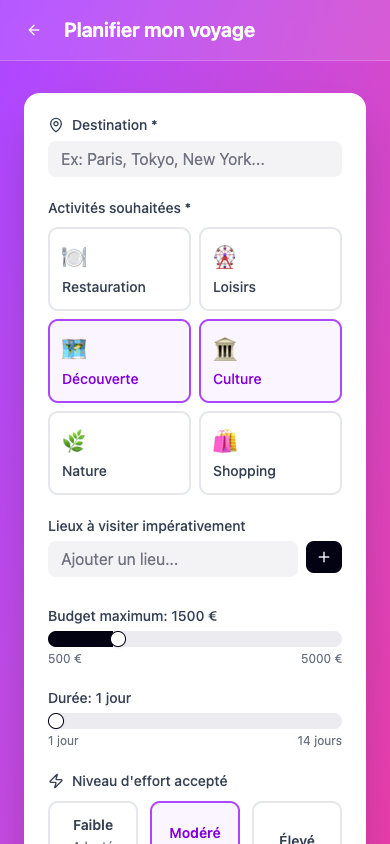
\includegraphics[width=0.95\textwidth]{sc_travelpath.png}
        \caption{Saisie critères}
    \end{minipage}\hfill
    \begin{minipage}{0.31\textwidth}
        \centering
        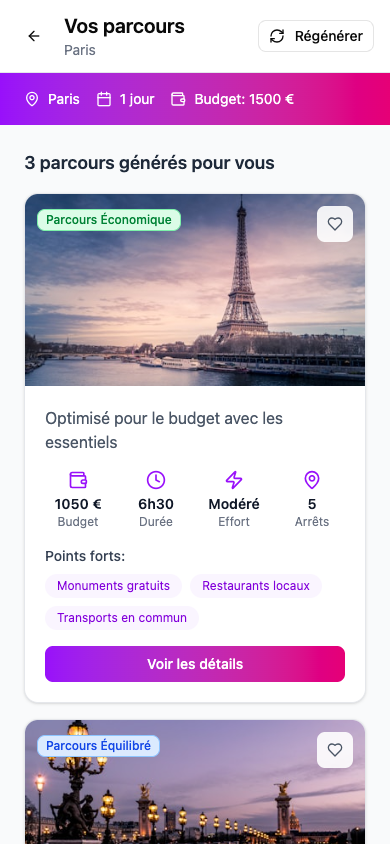
\includegraphics[width=0.95\textwidth]{sc_itinerary_options.png}
        \caption{Options}
    \end{minipage}\hfill
    \begin{minipage}{0.31\textwidth}
        \centering
        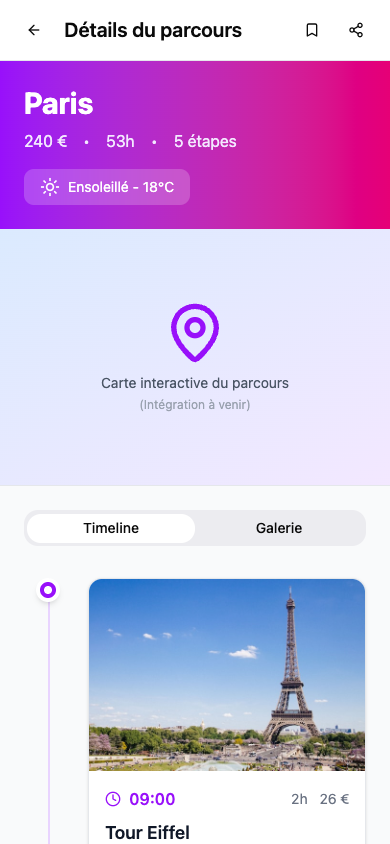
\includegraphics[width=0.95\textwidth]{sc_itinerary_detail.png}
        \caption{Détail et Carte}
    \end{minipage}
\end{figure}

\end{document}
